\documentclass[pdf]{prosper}

\usepackage[T1]{fontenc}
\usepackage[utf8]{inputenc}
\usepackage{amsmath}
\usepackage{amssymb}
\usepackage[table]{xcolor}
\usepackage{booktabs}
\usepackage{tikz}
\usetikzlibrary{positioning,calc,shapes.geometric,arrows.meta,backgrounds}
\usepackage[most]{tcolorbox}

\definecolor{deepnavy}{RGB}{27,38,59}
\definecolor{slateblue}{RGB}{65,90,119}
\definecolor{amber}{RGB}{224,159,62}
\definecolor{softgray}{RGB}{119,141,169}
\definecolor{paperwhite}{RGB}{247,247,245}

\newcommand{\Divider}[1]{%
\begin{slide}{}
\vspace{2.2cm}
\begin{center}
{\color{softgray}\rule{6cm}{0.4pt}}\\[0.5cm]
{\usefont{T1}{phv}{b}{n}\selectfont\color{deepnavy}\Huge #1}\\[0.4cm]
{\color{softgray}\rule{6cm}{0.4pt}}
\end{center}
\end{slide}%
}

\title{Adaptive Caching for Distributed Ledger Queries}
\subtitle{Cutting Read Latency in Permissioned Blockchain Networks \\[2pt]
\normalsize Meridian Symposium on Distributed Systems --- 2026}
\author{Dr.~Amara Voss \quad\&\quad Daniel Okafor}
\institution{Vertex University --- Department of Computer Science \\ Synapse Institute for Distributed Systems}
\email{a.voss@vertex.edu}
\slideCaption{Adaptive Caching for Distributed Ledger Queries}

\begin{document}

\maketitle

\begin{slide}{Agenda}
\vspace{0.4cm}
\begin{enumerate}
\item \textcolor{deepnavy}{\textbf{Motivation}} --- why read latency is a first-class problem
\item \textcolor{deepnavy}{\textbf{Background \& Related Work}} --- what existing caches miss
\item \textcolor{deepnavy}{\textbf{System Design}} --- the immutability-aware cache
\item \textcolor{deepnavy}{\textbf{Evaluation}} --- three production-shaped workloads
\item \textcolor{deepnavy}{\textbf{Discussion}} --- where the approach does and does not help
\item \textcolor{deepnavy}{\textbf{Conclusion}} --- results and open questions
\end{enumerate}
\vfill
{\small\color{softgray} Slides and the reference implementation will be released after the talk.}
\end{slide}

\Divider{Motivation}

\begin{slide}{Why Ledger Reads Are Slow}
\begin{itemize}
\item Permissioned ledgers used for internal settlement (e.g.\ the pilot network run by Apex Settlement Network) are read-heavy: audits, dashboards, and reconciliation jobs dominate traffic.
\item Every read --- even for a block finalized months ago --- re-walks the Merkle proof against the current ledger node state.
\item At Apex's pilot deployment, median query latency sat at \textbf{210\,ms} under \textbf{4{,}000 qps}, almost entirely proof-verification overhead.
\item \textbf{Goal:} cut tail latency substantially without weakening the ledger's consistency guarantees.
\end{itemize}
\vspace{0.5cm}
\begin{tcolorbox}[colback=paperwhite,colframe=slateblue,boxrule=0.6pt,arc=2pt,left=8pt,right=8pt,top=6pt,bottom=6pt]
\textbf{\textcolor{deepnavy}{Key observation:}} once a block is finalized in a permissioned network, its content is \emph{permanently} valid --- nothing about a historical read result can change.
\end{tcolorbox}
\end{slide}

\Divider{Background \& Related Work}

\begin{slide}{What Existing Caches Miss}
\begin{minipage}[t]{0.56\linewidth}
\begin{itemize}
\item \textbf{Read-through caches} (Redis-backed) treat every key as equally volatile and apply uniform TTLs.
\item \textbf{CDN-style edge caches} help static assets but do not understand block finality or reorg semantics.
\item \textbf{Application-level memoization} is ad hoc, duplicated across teams, and invalidated too conservatively.
\end{itemize}
\end{minipage}%
\hfill
\begin{minipage}[t]{0.38\linewidth}
\begin{tcolorbox}[colback=deepnavy,colframe=deepnavy,coltext=paperwhite,arc=2pt,left=6pt,right=6pt,top=6pt,bottom=6pt]
\textbf{Gap}\\[2pt]
\small No prior system exploits block \emph{immutability} as a caching invariant.
\end{tcolorbox}
\end{minipage}
\par
\vspace{0.6cm}
\textbf{Our idea:} a two-tier cache keyed by \((\text{block height}, \text{query type})\), invalidated only on the rare reorg event rather than on a timer.
\end{slide}

\Divider{System Design}

\begin{slide}{The Immutability-Aware Cache}
\begin{itemize}
\item The \textbf{Query Router} classifies each request as \emph{historical} (below the finality horizon, cacheable) or \emph{tip} (recent, still volatile).
\item Historical queries are served from the \textbf{Nimbus Cache Layer}, a write-once LRU keyed by block height and query type.
\item Tip queries bypass the cache entirely and go straight to the ledger nodes.
\item Cache entries warm lazily on first miss and never expire --- they are only evicted on an explicit reorg-invalidation sweep, which is rare by construction in permissioned settings.
\end{itemize}
\end{slide}

\begin{slide}{Request Flow}
\begin{center}
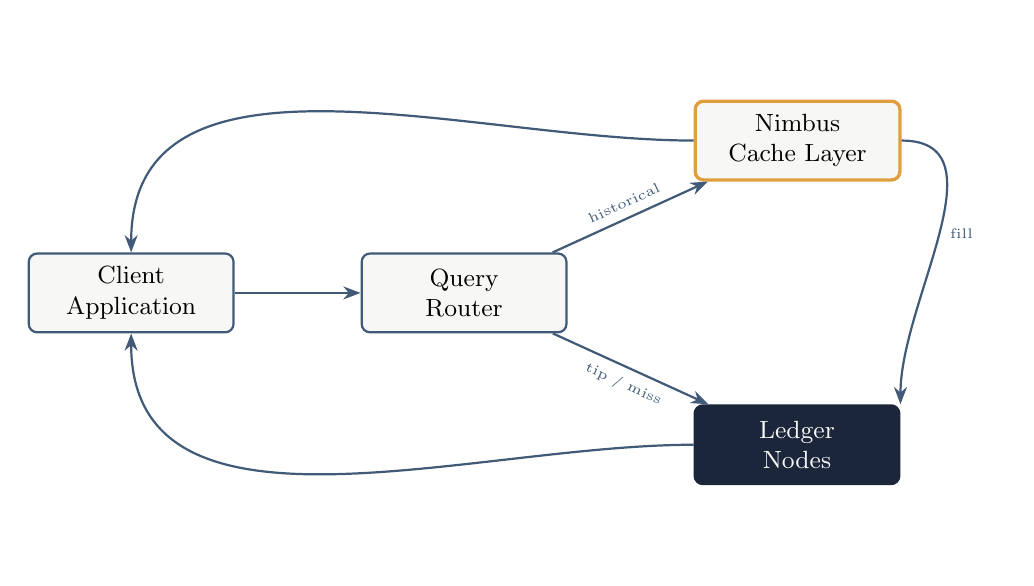
\begin{tikzpicture}[
  node distance=1.1cm and 1.6cm,
  box/.style={draw=slateblue, thick, rounded corners=3pt, fill=paperwhite, minimum height=1.0cm, minimum width=2.6cm, align=center, font=\small},
  cache/.style={draw=amber, very thick, rounded corners=3pt, fill=paperwhite, minimum height=1.0cm, minimum width=2.6cm, align=center, font=\small},
  ledger/.style={draw=deepnavy, thick, rounded corners=3pt, fill=deepnavy, text=paperwhite, minimum height=1.0cm, minimum width=2.6cm, align=center, font=\small},
  arr/.style={-{Stealth[length=2.2mm]}, thick, slateblue}
]
\node[box] (client) {Client\\Application};
\node[box, right=of client] (router) {Query\\Router};
\node[cache, above right=0.9cm and 1.6cm of router] (cache) {Nimbus\\Cache Layer};
\node[ledger, below right=0.9cm and 1.6cm of router] (ledger) {Ledger\\Nodes};

\draw[arr] (client) -- (router);
\draw[arr] (router) -- node[above, sloped, font=\tiny] {historical} (cache);
\draw[arr] (router) -- node[below, sloped, font=\tiny] {tip / miss} (ledger);
\draw[arr] (cache.east) to[out=0,in=90] node[right, font=\tiny] {fill} (ledger.north east);
\draw[arr] (cache) to[out=180,in=90] (client.north);
\draw[arr] (ledger) to[out=180,in=270] (client.south);
\end{tikzpicture}
\end{center}
\vspace{0.2cm}
{\small\color{softgray} Historical reads terminate at the cache; only misses and tip reads touch a ledger node.}
\end{slide}

\Divider{Evaluation}

\begin{slide}{Experimental Setup}
\begin{itemize}
\item \textbf{Testbed:} 12-node permissioned network across 3 emulated regions, running the Nimbus Cache Layer prototype in front of unmodified ledger nodes.
\item \textbf{Baseline:} direct ledger-node reads with full Merkle re-verification on every query.
\item \textbf{Workloads:}
\begin{itemize}
\item \textbf{W1 --- Audit Replay:} 99\% historical reads, replaying six months of settlement records.
\item \textbf{W2 --- Mixed Dashboard:} 70\% historical, 30\% tip, matching Apex's internal reporting tool.
\item \textbf{W3 --- Live Monitoring:} 10\% historical, 90\% tip --- a near-real-time alerting workload.
\end{itemize}
\end{itemize}
\end{slide}

\begin{slide}{Results}
\begin{center}
\renewcommand{\arraystretch}{1.25}
\resizebox{\linewidth}{!}{%
\begin{tabular}{lccc}
\toprule
\textbf{Workload} & \textbf{Baseline p50 (ms)} & \textbf{Adaptive p50 (ms)} & \textbf{Hit Rate (\%)} \\
\midrule
\rowcolor{paperwhite} W1 --- Audit Replay & 198 & 11 & 97 \\
W2 --- Mixed Dashboard & 205 & 64 & 71 \\
\rowcolor{paperwhite} W3 --- Live Monitoring & 212 & 189 & 9 \\
\bottomrule
\end{tabular}
}%
\end{center}
\vspace{0.4cm}
\begin{tcolorbox}[colback=paperwhite,colframe=amber,boxrule=0.8pt,arc=2pt,left=8pt,right=8pt,top=6pt,bottom=6pt]
\textbf{\textcolor{deepnavy}{Headline:}} up to \textbf{17$\times$} lower median latency on audit-shaped traffic, with zero consistency compromise.
\end{tcolorbox}
\end{slide}

\Divider{Discussion}

\begin{slide}{Limitations \& Threats to Validity}
\begin{itemize}
\item Gains concentrate where the historical fraction is high; W3's live-monitoring traffic barely benefits, which is expected since it targets the volatile tip by design.
\item Reorg handling adds a small invalidation-sweep cost --- negligible in our traces, but not yet stress-tested under adversarial conditions.
\item We have not evaluated behavior under Byzantine node faults or deliberately induced reorgs.
\item Results are drawn from one permissioned deployment; generalization to other governance models is untested.
\end{itemize}
\end{slide}

\Divider{Conclusion}

\begin{slide}{Conclusion \& Future Work}
\begin{itemize}
\item Treating block immutability as a first-class caching invariant cuts median latency by up to 17$\times$ on audit- and reporting-shaped workloads.
\item The two-tier router/cache split requires no changes to existing ledger-node code.
\item \textbf{Future work:} extend the router to cross-shard queries, and explore access-pattern-driven prefetching for the cache layer.
\item \textbf{Open question:} does the same invariant --- and the same speedup --- hold for public chains with only probabilistic finality?
\end{itemize}
\end{slide}

\begin{slide}{Acknowledgments}
\begin{itemize}
\item Funded in part by a \textbf{Nimbus Research Foundation} grant.
\item Compute infrastructure provided by the \textbf{Synapse Institute} cluster.
\item Thanks to the engineering team at \textbf{Apex Settlement Network} for sharing production traces.
\end{itemize}
\end{slide}

\begin{slide}{}
\vspace{2.0cm}
\begin{center}
{\usefont{T1}{phv}{b}{n}\selectfont\color{deepnavy}\Huge Thank You}\\[0.6cm]
{\color{slateblue}\Large Questions \& Discussion}\\[1.0cm]
{\small\color{softgray}
Dr.~Amara Voss \quad$\cdot$\quad a.voss@vertex.edu\\
Vertex University --- Department of Computer Science}
\end{center}
\end{slide}

\end{document}
